% 固定来源PDF印刷页51第23题圆柱、轴截面和垂足的示意重绘。
% 图中比例仅作示意，不添加题干未给出的度量条件。
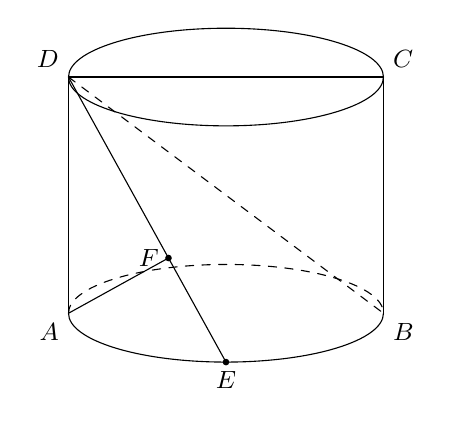
\begin{tikzpicture}[x=1cm,y=1cm,font=\small,line cap=round,line join=round]
  \coordinate (A) at (0,0);
  \coordinate (B) at (4,0);
  \coordinate (C) at (4,3);
  \coordinate (D) at (0,3);
  \coordinate (E) at (2,-.62);
  % F is the orthogonal projection of A onto DE in this schematic.
  \coordinate (F) at (1.269849,.701574);

  % Cylinder surface and circular rims; back half of the lower rim is hidden.
  \draw (D)--(A) (C)--(B);
  \draw (D)--(C);
  \draw (2,3) ellipse (2 and .62);
  \draw[dashed] (A) arc[start angle=180,end angle=0,x radius=2,y radius=.62];
  \draw (A) arc[start angle=180,end angle=360,x radius=2,y radius=.62];
  % Axial-section diagonal, DE and its perpendicular AF.
  \draw[dashed] (D)--(B);
  \draw (D)--(E) (A)--(F);
  \fill (E) circle (1.2pt) (F) circle (1.2pt);

  \node[above left] at (D) {$D$};
  \node[above right] at (C) {$C$};
  \node[below left] at (A) {$A$};
  \node[below right] at (B) {$B$};
  \node[below] at (E) {$E$};
  \node[left] at (F) {$F$};
\end{tikzpicture}
